% Figure: the research design of the proposal. Four steps of design science,
% the output of each step, and the research question that each step serves.
% Standalone TikZ source. The colors match the figures of the manuscript.
\documentclass[tikz,border=2pt]{standalone}
\usetikzlibrary{arrows.meta,calc,positioning}

\definecolor{ink}{HTML}{0B0B0B}
\definecolor{inksoft}{HTML}{52514E}
\definecolor{muted}{HTML}{898781}
\definecolor{phasefill}{HTML}{CDE2FB}
\definecolor{phaseborder}{HTML}{1C5CAB}
\definecolor{questionfill}{HTML}{FBE1D6}
\definecolor{questionborder}{HTML}{B8501F}

\begin{document}
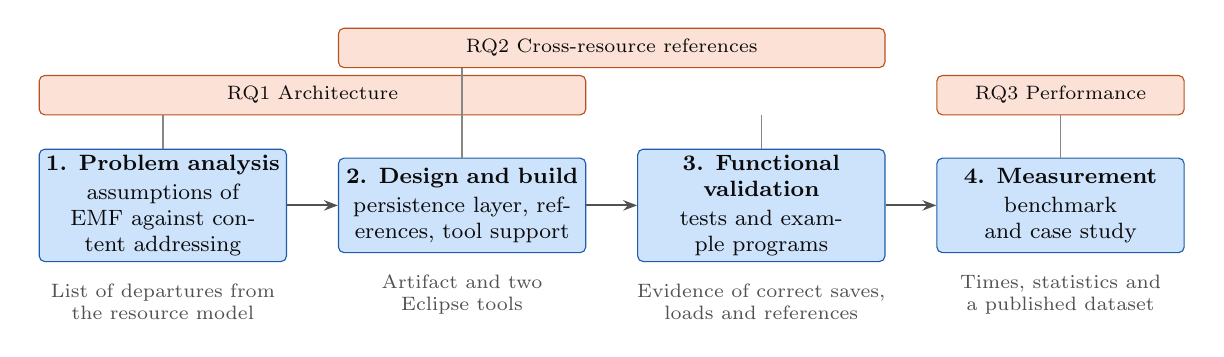
\begin{tikzpicture}[
  font=\footnotesize,
  >={Stealth[length=5pt]},
  phase/.style={draw=phaseborder, fill=phasefill, rounded corners=2pt, text=ink,
    align=center, text width=30mm, minimum height=12mm, inner sep=2pt},
  outnote/.style={text=inksoft, font=\scriptsize, align=center, text width=32mm, anchor=north},
  question/.style={draw=questionborder, fill=questionfill, rounded corners=2pt, text=ink,
    align=center, minimum height=5mm, inner sep=2pt, font=\scriptsize},
  flow/.style={->, draw=inksoft, line width=0.7pt}
]

\node[phase] (s1) at (0,0) {\textbf{1. Problem analysis}\\[1pt] assumptions of EMF against content addressing};
\node[phase] (s2) at (38mm,0) {\textbf{2. Design and build}\\[1pt] persistence layer, references, tool support};
\node[phase] (s3) at (76mm,0) {\textbf{3. Functional validation}\\[1pt] tests and example programs};
\node[phase] (s4) at (114mm,0) {\textbf{4. Measurement}\\[1pt] benchmark and case study};

\draw[flow] (s1) -- (s2);
\draw[flow] (s2) -- (s3);
\draw[flow] (s3) -- (s4);

\node[outnote] at ($(s1.south)+(0,-1.5mm)$) {List of departures from the resource model};
\node[outnote] at ($(s2.south)+(0,-1.5mm)$) {Artifact and two Eclipse tools};
\node[outnote] at ($(s3.south)+(0,-1.5mm)$) {Evidence of correct saves, loads and references};
\node[outnote] at ($(s4.south)+(0,-1.5mm)$) {Times, statistics and a published dataset};

\node[question, text width=68mm] (rq1) at (19mm,14mm) {RQ1 Architecture};
\node[question, text width=68mm] (rq2) at (57mm,20mm) {RQ2 Cross-resource references};
\node[question, text width=30mm] (rq3) at (114mm,14mm) {RQ3 Performance};

\draw[draw=muted, line width=0.5pt] (s1.north) -- (s1.north|-rq1.south);
\draw[draw=muted, line width=0.5pt] (s3.north) -- (s3.north|-rq1.south);
\draw[draw=muted, line width=0.5pt] (s2.north) -- (s2.north|-rq2.south);
\draw[draw=muted, line width=0.5pt] (s4.north) -- (s4.north|-rq3.south);
\end{tikzpicture}
\end{document}
